\documentclass[main.tex]{subfiles}

\begin{document}
    \justifying

    \section{Performance analysis}
    \label{section:performance-analysis}
       
        In this section, we highlight the results from a comprehensive performance testing. We compare the developed CLOUDSC-GT4Py and CLOUDSC2-GT4Py codes against reference Fortran versions and various other programming prototypes. The simulations were performed on three different supercomputers: 
        \begin{itemize}
            \item[(i)] Piz Daint\footnote{\url{https://www.cscs.ch/computers/piz-daint}}, an HPE Cray XC40/XC50 system installed at CSCS in Lugano, Switzerland;
            \item[(ii)] MeluXina\footnote{\url{https://docs.lxp.lu/}}, an ATOS BullSequana XH2000 machine hosted by LuxConnect in Bissen, Luxembourg, and procured by the EuroHPC Joint Undertaking (JU) initiative;
            \item[(iii)] the Cray HPE EX235a supercomputer LUMI\footnote{\url{https://docs.lumi-supercomputer.eu/}}, an EuroHPC pre-exascale machine at the Science Information Technology Center (CSC) in Kajaani, Finland.
        \end{itemize} 
        On each machine, the CLOUDSC and CLOUDSC2 applications are executed on a single hybrid node, that sports one or multiple GPU accelerators alongside the host CPU. An overview of the node architectures for the three considered supercomputers can be found in Table \ref{tab:architecture}. 

        \begin{table}[t!]
            \setlength\extrarowheight{2pt}
            \centering
            \begin{tabular}{|c|c|c|c|c|}
                 \hline
                 \textbf{System} & \textbf{CPU} & \textbf{GPU} & \textbf{RAM} & \textbf{NUMA domains} \\
                 \hline
                 Piz Daint & 1x Intel Xeon E5-2690v3 12c & 1x NVIDIA Tesla P100 16GB & 64 GB & 1 \\
                 MeluXina & 2x AMD EPYC Rome 7452 32c & 4x NVIDIA Tesla A100 40GB & 512 GB & 4 \\
                 LUMI & 1x AMD EPYC Trento 7A53 64c & 4x AMD Instinct MI250X & 512 GB & 8 \\
                 \hline
            \end{tabular}
            \vspace*{0.2cm}
            \caption{Overview of the node architecture for the hybrid partition of Piz Daint, MeluXina and LUMI. Only the technical specifications which are most relevant for the purposes of this paper are reported.}
            \label{tab:architecture}
        \end{table}
        
        Besides the GT4Py codes, we involve up to four alternative lower-level programming implementations, which will be documented in an upcoming publication.
        \begin{itemize}
            \item[(a)] The baseline Fortran version, enriched with OpenMP directives for multi-threading execution on CPU.
            \item[(b)] An optimized GPU-enabled version based on OpenACC using the single-column coalesced (SCC) loop layout in combination with loop fusion and temporary local array demotion (so-called ``k-caching''). While the SCC loop layout yields more efficient access to device memory and increased parallelism, the k-caching technique significantly reduces register pressure and memory traffic. This is achieved via loop fusion to eliminate most loop-carried dependencies and consequently allows to demote temporaries to scalars.
            \item[(c)] The currently best-performing Loki generated and GPU-enabled variant.
            \item[(d)] An optimized GPU-enabled version of CLOUDSC including k-caching. The code is written either in CUDA or HIP, to target both NVIDIA GPUs (shipped with Piz Daint and MeluXina) and AMD GPUs (available on LUMI).
        \end{itemize}

        \begin{table}[t!]
            \renewcommand{\arraystretch}{1.4}
            \centering
            \begin{footnotesize}
                \begin{tabular}{|c|c|c|c|c|}
                     \hline
                     & \textbf{Implementation} & \textbf{CLOUDSC} & \textbf{CLOUDSC2: Non-linear} & \textbf{CLOUDSC2: Symmetry test} \\
                     \hline
                     \multirow{6}{*}{\rotatebox[origin=c]{90}{\textbf{Piz Daint}}} & Fortran: OpenMP (CPU) & Intel Fortran 2021.3.0 & Intel Fortran 2021.3.0 & Intel Fortran 2021.3.0 \\
                     & Fortran: OpenACC (GPU) & NVIDIA Fortran 21.3-0 & - & - \\
                     & Fortran: Loki (GPU) & NVIDIA Fortran 21.3-0 & NVIDIA Fortran 21.3-0 & - \\
                     & C: CUDA (GPU) & NVIDIA CUDA 11.2.67 & - & - \\
                     & GT4Py: CPU k-first & g++ (GCC) 10.3.0 & g++ (GCC) 10.3.0 & g++ (GCC) 10.3.0 \\
                     & GT4Py: DaCe (GPU) & NVIDIA CUDA 11.2.67 & NVIDIA CUDA 11.2.67 & NVIDIA CUDA 11.2.67 \\
                     \hline
                     \multirow{6}{*}{\rotatebox[origin=c]{90}{\textbf{MeluXina}}} & Fortran: OpenMP (CPU) & NVIDIA Fortran 22.7-0 & NVIDIA Fortran 22.7-0 & - \\
                     & Fortran: OpenACC (GPU) & NVIDIA Fortran 22.7-0 & - & - \\
                     & Fortran: Loki (GPU) & NVIDIA Fortran 22.7-0 & NVIDIA Fortran 22.7-0 & - \\
                     & C: CUDA (GPU) & NVIDIA CUDA 11.7.64 & - & - \\
                     & GT4Py: CPU k-first & g++ (GCC) 11.3.0 & g++ (GCC) 11.3.0 & g++ (GCC) 11.3.0 \\
                     & GT4Py: DaCe (GPU) & NVIDIA CUDA 11.7.64 & NVIDIA CUDA 11.7.64 & NVIDIA CUDA 11.7.64 \\
                     \hline
                     \multirow{6}{*}{\rotatebox[origin=c]{90}{\textbf{LUMI}}} & Fortran: OpenMP (CPU) & ~~ Cray Fortran 14.0.2 ~~ & Cray Fortran 14.0.2 & Cray Fortran 14.0.2 \\
                     & Fortran: OpenACC (GPU) & Cray Fortran 14.0.2 & - & - \\
                     & Fortran: Loki (GPU) & Cray Fortran 14.0.2 & Cray Fortran 14.0.2 & - \\
                     & C: HIP (GPU) & Cray C/C++ 15.0.1 & - & - \\
                     & GT4Py: CPU k-first & Cray C/C++ 15.0.1 & Cray C/C++ 15.0.1 & Cray C/C++ 15.0.1 \\
                     & GT4Py: DaCe (GPU) & Cray C/C++ 15.0.1 & Cray C/C++ 15.0.1 & Cray C/C++ 15.0.1 \\
                     \hline
                \end{tabular}
            \end{footnotesize}
            \vspace*{0.2cm}
            \caption{For each coding version of the CLOUDSC and CLOUDSC2 dwarfs considered in the performance analysis, the table reports the compiler suite used to compile the codes on Piz Daint, MeluXina and LUMI. The codes are compiled with all major optimization options enabled. Those implementations which are either not available or not working are marked with a dash; more details, as well as a high-level description of each coding implementation, are provided in the text.}
            \label{tab:compiler}
        \end{table}
        
        \noindent Table \ref{tab:compiler} documents the compiler specifications employed for each of the programming implementations, on Piz Daint, MeluXina and LUMI. We consistently apply the most aggressive optimization, ensuring that the underlying code manipulations do not harm validation. For the different algorithms at consideration, validation is carried out as follows.
        \begin{itemize}
            \item For CLOUDSC and CLOUDSC2NL, the results from each coding version are directly compared with serialized reference data produced on the CPU. For each output field, we perform an element-wise comparison using the NumPy function \pyinline{allclose}\footnote{\url{https://numpy.org/devdocs/reference/generated/numpy.allclose.html}}. Specifically, the GT4Py rewrites validate on both CPU and GPU with an absolute and relative tolerance of $10^{-12}$ and $10^{-18}$ when employing double precision. When reducing the precision to 32-bits, the absolute and relative tolerance levels need to be increased to $10^{-4}$ and $10^{-7}$ on CPU, and $10^{-2}$ and $10^{-7}$ on GPU. In the latter case, we observe that the field representing the enthalpy flux of ice still does not pass validation. We attribute the larger deviation from the baseline data on the device to the different instruction sets underneath CPUs and GPUs.
            \item All implementations of CLOUDSC2TL and CLOUDSC2AD are validated using the Taylor test (cf.\,Algorithm \ref{alg:taylor-test}) and the symmetry test (cf.\,Algorithm \ref{alg:symmetry-test}), respectively. In this respect, we emphasize that the GT4Py implementations satisfy the conditions of both tests on all considered computing architectures, regardless of whether double or single precision is employed.
        \end{itemize}
        \noindent The source repositories for CLOUDSC and CLOUDSC2 dwarfs may include multiple variants of each reference implementation, varying for the optimization strategies. In our analysis, we always take into account the fastest variant of each alternative implementation; for the sake of reproducibility, Table \ref{tab:versions} contains the strings identifying the coding versions at consideration and the corresponding NPROMA\footnote{NPROMA slicing is a cache blocking technique adopted in all Fortran codes considered in this paper. Given a two-dimensional array shaped $(K * M, \, N)$, this is re-arranged as a three-dimensional array shaped $(K, \, M, \, N)$. The leading dimension of the three-dimensional array is commonly called ``NPROMA'', with $K$ being the ``NPROMA blocking factor''. For the sake of brevity, in the text we indicate $K$ simply as ``NPROMA''. For an insightful discussion on the NPROMA slicing technique, we refer the readers to, e.g., \citet{muller19} and \citet{bauer20}.} employed in the runs. Similarly, for all Python implementations we consider only the most performant backends of GT4Py: the GridTools C++ CPU backend with k-first memory layout, and the DaCe GPU backend.
        
        \begin{table}[t!]
            \renewcommand{\arraystretch}{1.4}
            \centering
            \begin{footnotesize}
                \begin{tabular}{|c|c|c|c|c|}
                     \hline
                     & \textbf{Implementation} & \textbf{CLOUDSC} & \textbf{CLOUDSC2: Non-linear} & \textbf{CLOUDSC2: Symmetry test} \\
                     \hline
                     \multirow{4}{*}{\rotatebox[origin=c]{90}{\textbf{Piz Daint}}} & Fortran: OpenMP (CPU) & \texttt{fortran} (32) & \texttt{nl} (32) & \texttt{ad} (32) \\
                     & Fortran: OpenACC (GPU) & \texttt{gpu-scc-k-caching} (128) & - & - \\
                     & Fortran: Loki (GPU) & \texttt{loki-scc-cuf-hoist} (128) & \texttt{nl-loki-scc-hoist} (64) & - \\
                     & C: CUDA (GPU) & \texttt{cuda-k-caching} (128) & - & - \\
                     \hline
                     \multirow{4}{*}{\rotatebox[origin=c]{90}{\textbf{MeluXina}}} & Fortran: OpenMP (CPU) & \texttt{fortran} (32) & \texttt{nl} (32) & - \\
                     & Fortran: OpenACC (GPU) & \texttt{gpu-scc-k-caching} (128) & - & - \\
                     & Fortran: Loki (GPU) & \texttt{loki-scc-cuf-hoist} (128) & \texttt{nl-loki-scc-hoist} (128) & - \\
                     & C: CUDA (GPU) & \texttt{cuda-k-caching} (128) & - & - \\
                     \hline
                     \multirow{4}{*}{\rotatebox[origin=c]{90}{\textbf{LUMI}}} & Fortran: OpenMP (CPU) & ~~ \texttt{fortran} (32) ~~ & \texttt{nl} (32) & \texttt{ad} (32) \\
                     & Fortran: OpenACC (GPU) & \texttt{gpu-scc-k-caching} (256) & - & - \\
                     & Fortran: Loki (GPU) & \texttt{loki-scc-hoist} (256) & \texttt{nl-loki-scc-hoist} (256) & - \\
                     & C: HIP (GPU) & \texttt{hip-k-caching} (64) & - & - \\
                     \hline
                \end{tabular}
            \end{footnotesize}
            \vspace*{0.2cm}
            \caption{For each reference implementation of the CLOUDSC and CLOUDSC2 dwarfs, the table reports the string identifying the specific variant considered in the performance analysis on Piz Daint, MeluXina and LUMI. The corresponding NPROMA is provided within parentheses. Those implementations which are either not available or not working are marked with a dash.}
            \label{tab:versions}
        \end{table}

        \begin{figure}[t!]
            \centering
            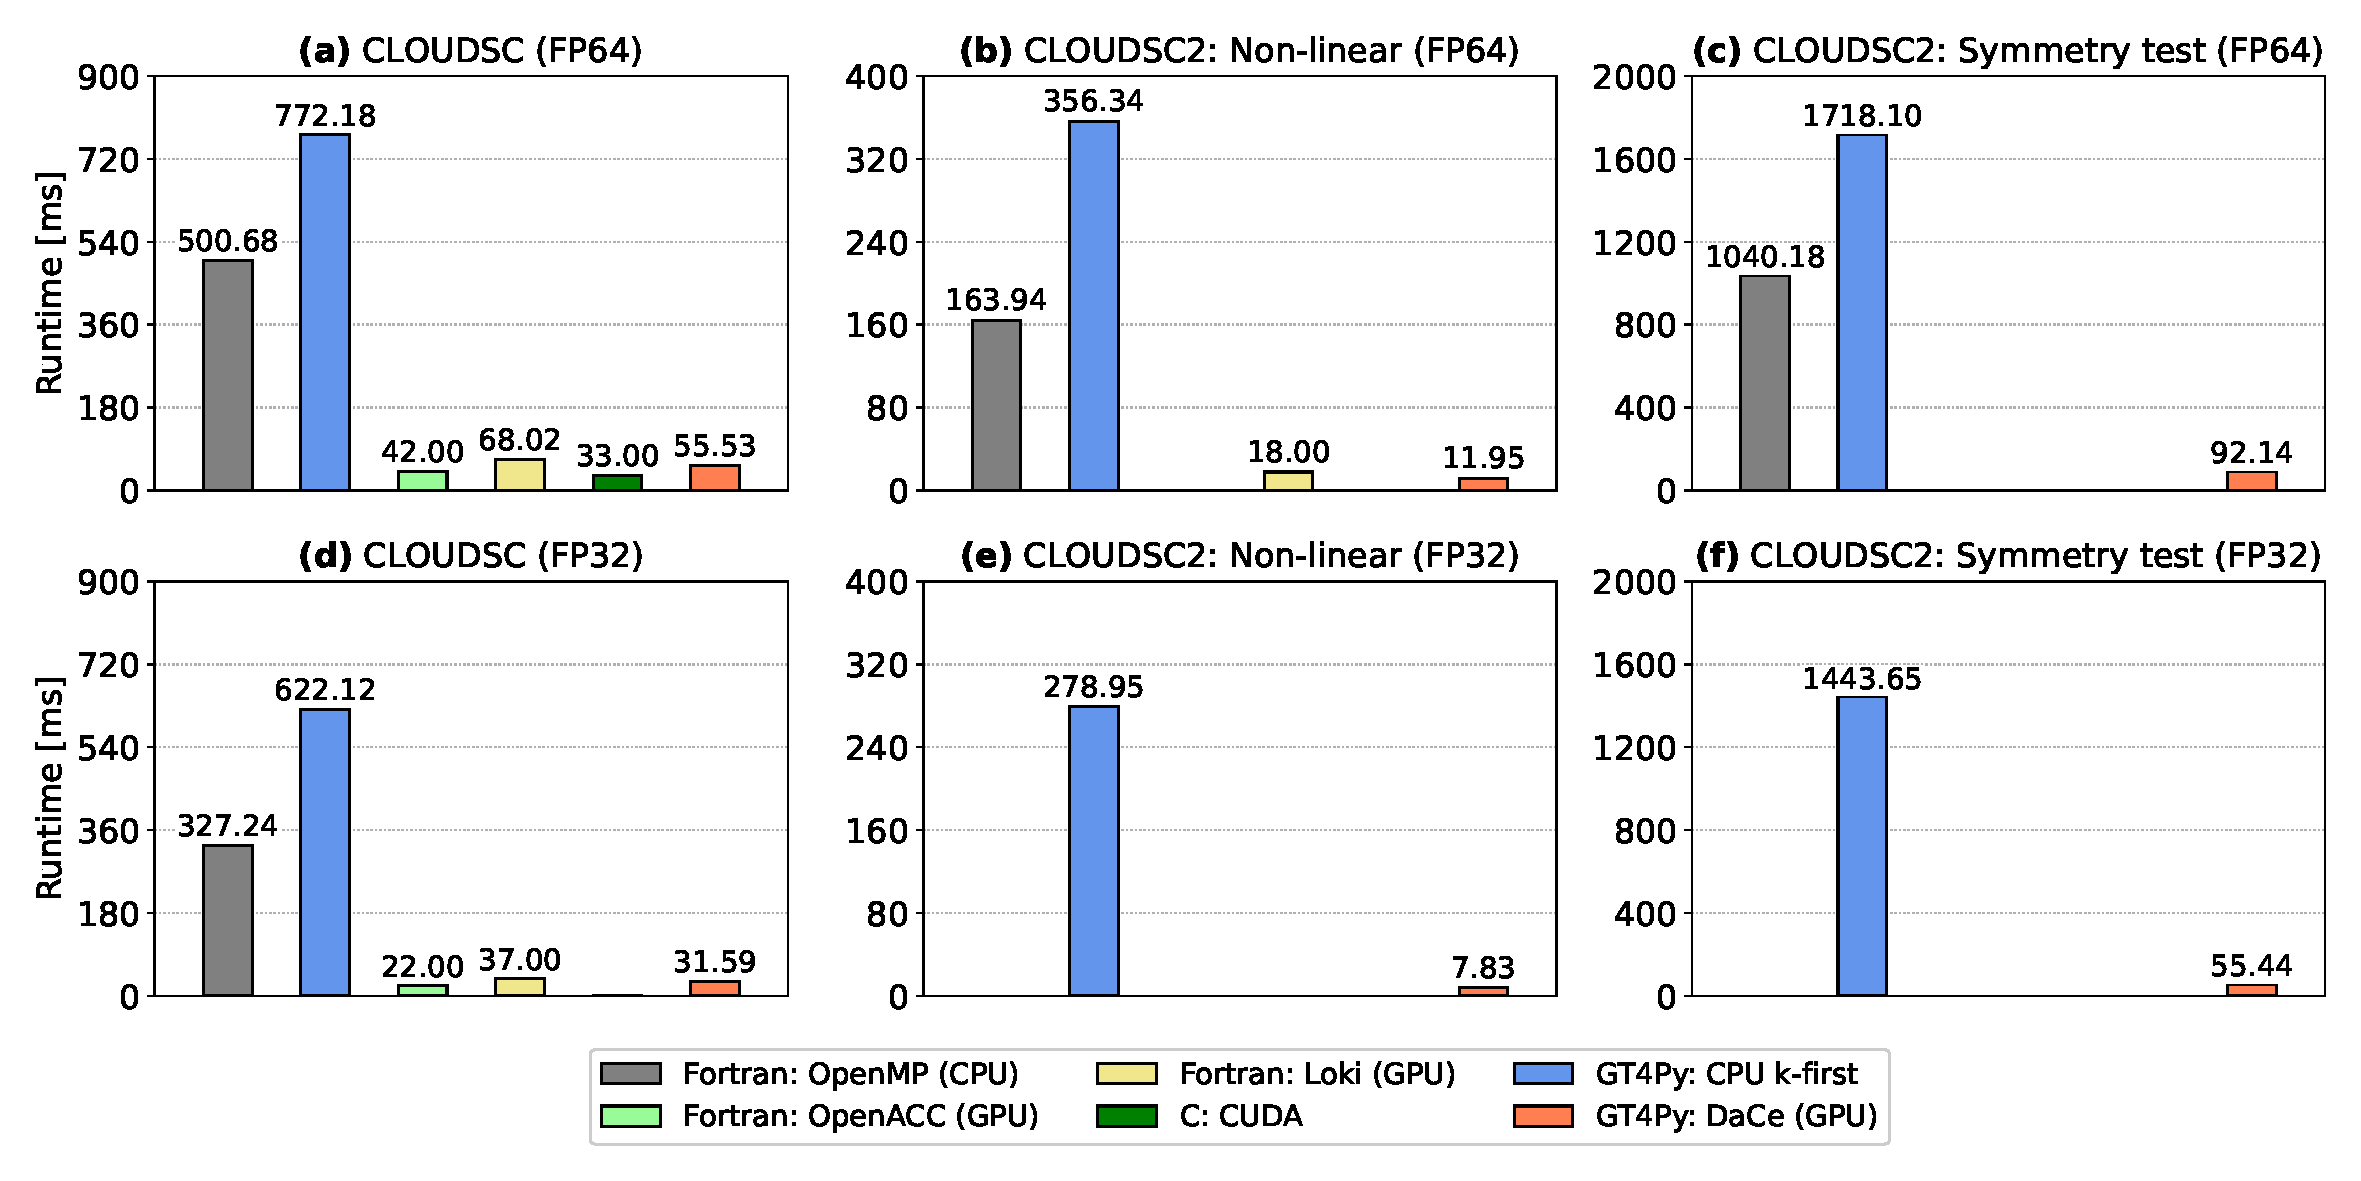
\includegraphics[scale=0.44]{performance_daint_2.pdf}
            \caption{Execution time on a single NUMA domain of a hybrid node of the Piz Daint supercomputer for CLOUDSC (left column), CLOUDSC2NL (center column) and the symmetry test for CLOUDSC2TL and CLOUDSC2AD (right column) using either double precision (top row) or single precision (bottom row) floating point arithmetic. The computational domain consists of 65536 columns and 137 vertical levels. Displayed are the multi-threaded Fortran baseline using OpenMP (grey); two GPU-accelerated Fortran implementations, either using OpenACC directives (lime) or the source-to-source translation tool Loki (yellow); an optimized CUDA C version (green); and the GT4Py rewrite, either using the GridTools C++ CPU backend with k-first data ordering (blue) or the DaCe GPU backend (orange). All numbers should be interpreted as an average over $50$ realizations. The panels only show the code versions available and validating at the time of writing.}
            \label{fig:performance-daint}
        \end{figure}
        
        \noindent For the interpretation of the CPU versus GPU performance numbers, we note that host codes are executed on all the cores available on a single Non-Uniform Memory Access (NUMA) domain of a compute node, while device codes are launched on the GPU attached to that NUMA domain. In a distributed-memory context, this choice allows to fit the same number of MPI ranks per node, either on CPU or GPU. Table \ref{tab:architecture} reports the number of NUMA partitions per node for Piz Daint, MeluXina and LUMI, with the compute and memory resources being evenly distributed across the NUMA domains. Note that the compute nodes of the GPU partition of LUMI have the low-noise mode activated, which reserves one core per NUMA domain to the operating system, so that only 7 out of 8 cores are available to the jobs. Moreover, we highlight that each MI250X GPU consists of two Graphics Compute Dies (GCDs) connected via four AMD Infinity Fabric links but not sharing physical memory. From a software perspective, each compute node of LUMI is equipped with 8 virtual GPUs (vGPUs), with each vGPU corresponding to a single GCD and assigned to a different NUMA domain.

        \begin{figure}[t!]
            \centering
            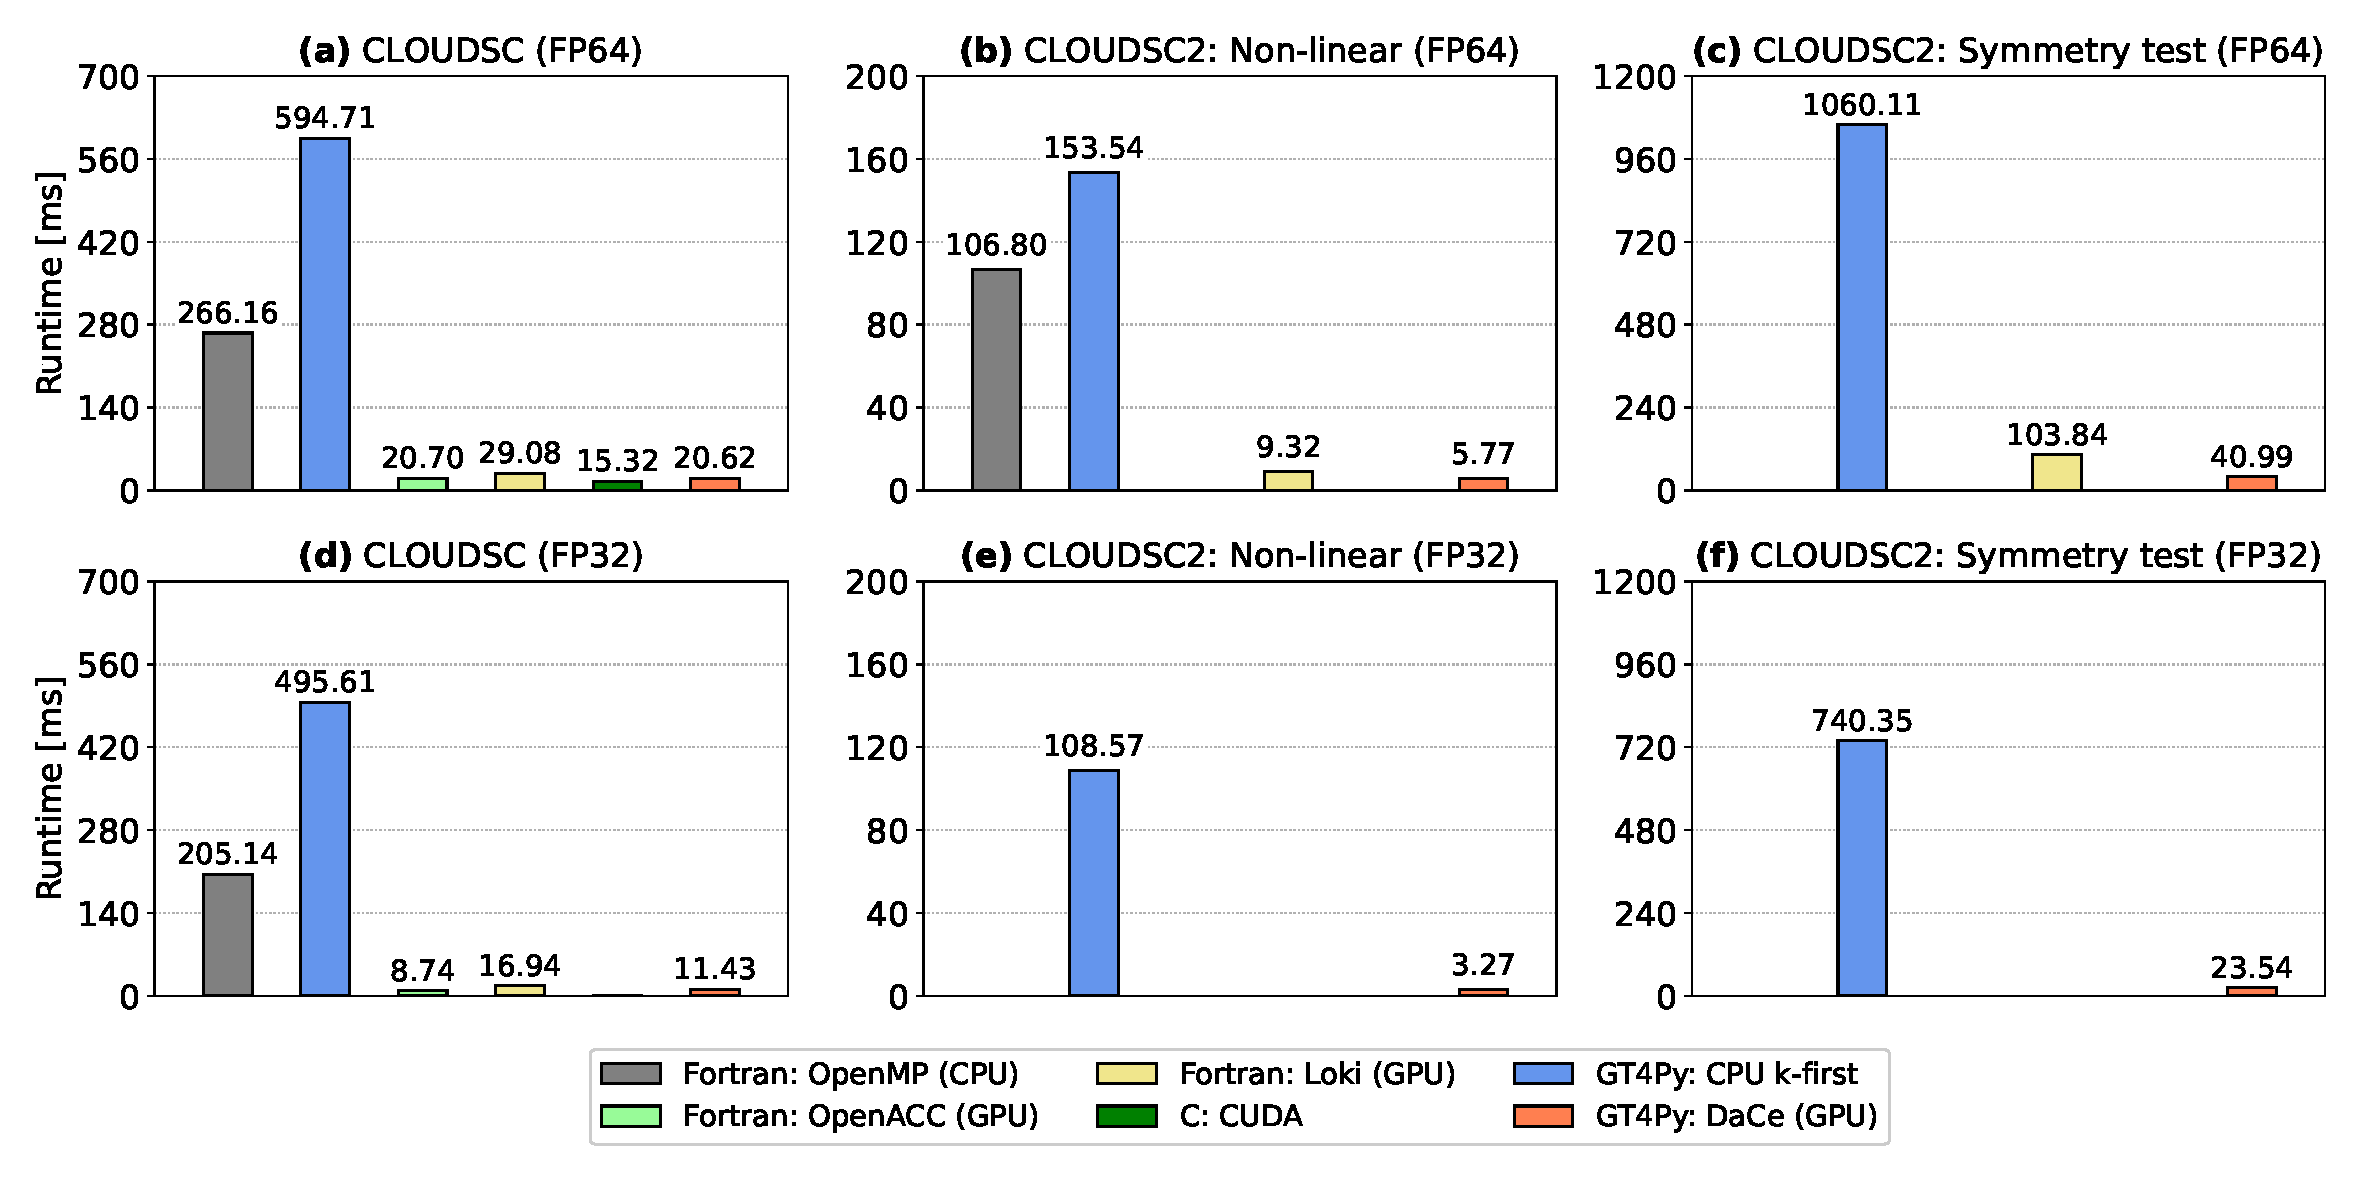
\includegraphics[scale=0.44]{performance_mlux_2.pdf}
            \caption{As Fig.\,\ref{fig:performance-daint} but for the MeluXina supercomputer.}
            \label{fig:performance-mlux}
        \end{figure}

        Figures \ref{fig:performance-daint}-\ref{fig:performance-lumi} visualize the execution times for CLOUDSC (left column), CLOUDSC2NL  (center column) and the symmetry test for CLOUDSC2TL and CLOUDSCAD (right column) for Piz Daint, MeluXina and LUMI, respectively\footnote{When measuring the performance of the symmetry test, the validation procedure -- corresponding to lines 11-23 of Algorithm \ref{alg:symmetry-test} -- is switched off.}. All performance numbers refer to a grid size of 65536 columns, with each column featuring 137 vertical levels. In each figure, execution times are provided for simulations running either entirely in double precision (corresponding to the 64-bit IEEE format and denoted as FP64; top row) or in single precision (corresponding to the 32-bit IEEE format and denoted as FP32; bottom row). Within each panel, the plotted bars reflect the execution time of the various codes, with a missing bar indicating the corresponding code (non-GT4Py) is either not available or not working properly. Specifically,
        \begin{itemize}
            \item the Fortran version of CLOUDSC2AD can only run on a single OpenMP thread on MeluXina (the issue is still under investigation);
            \item a native GPU-enabled version of CLOUDSC using 32-bit floating point arithmetic does not exist at the time of writing, and no CUDA/HIP implementations are available for CLOUDSC2;
            \item all Fortran-based implementations of the three formulations of CLOUDSC2 can only use double precision computations;
            \item a Loki version of CLOUDSC2TL and CLOUDSC2AD is not available at the time of writing.
        \end{itemize}
        
        \noindent Notably, we find the GT4Py rewrite of both CLOUDSC and CLOUDSC2 to be very robust, as the codes execute on every CPU and GPU architecture included in the study, and can always employ either double or single precision floating point arithmetic. With GT4Py, changing the backend with the respective target architecture, or changing the precision of computations, is as easy as setting a namelist parameter. Moreover, at the time of writing the GT4Py implementations of the more complex tangent-linear and adjoint formulations of CLOUDSC2 were the first codes enabling GPU execution, again both in double or single precision.

        \begin{figure}[t!]
            \centering
            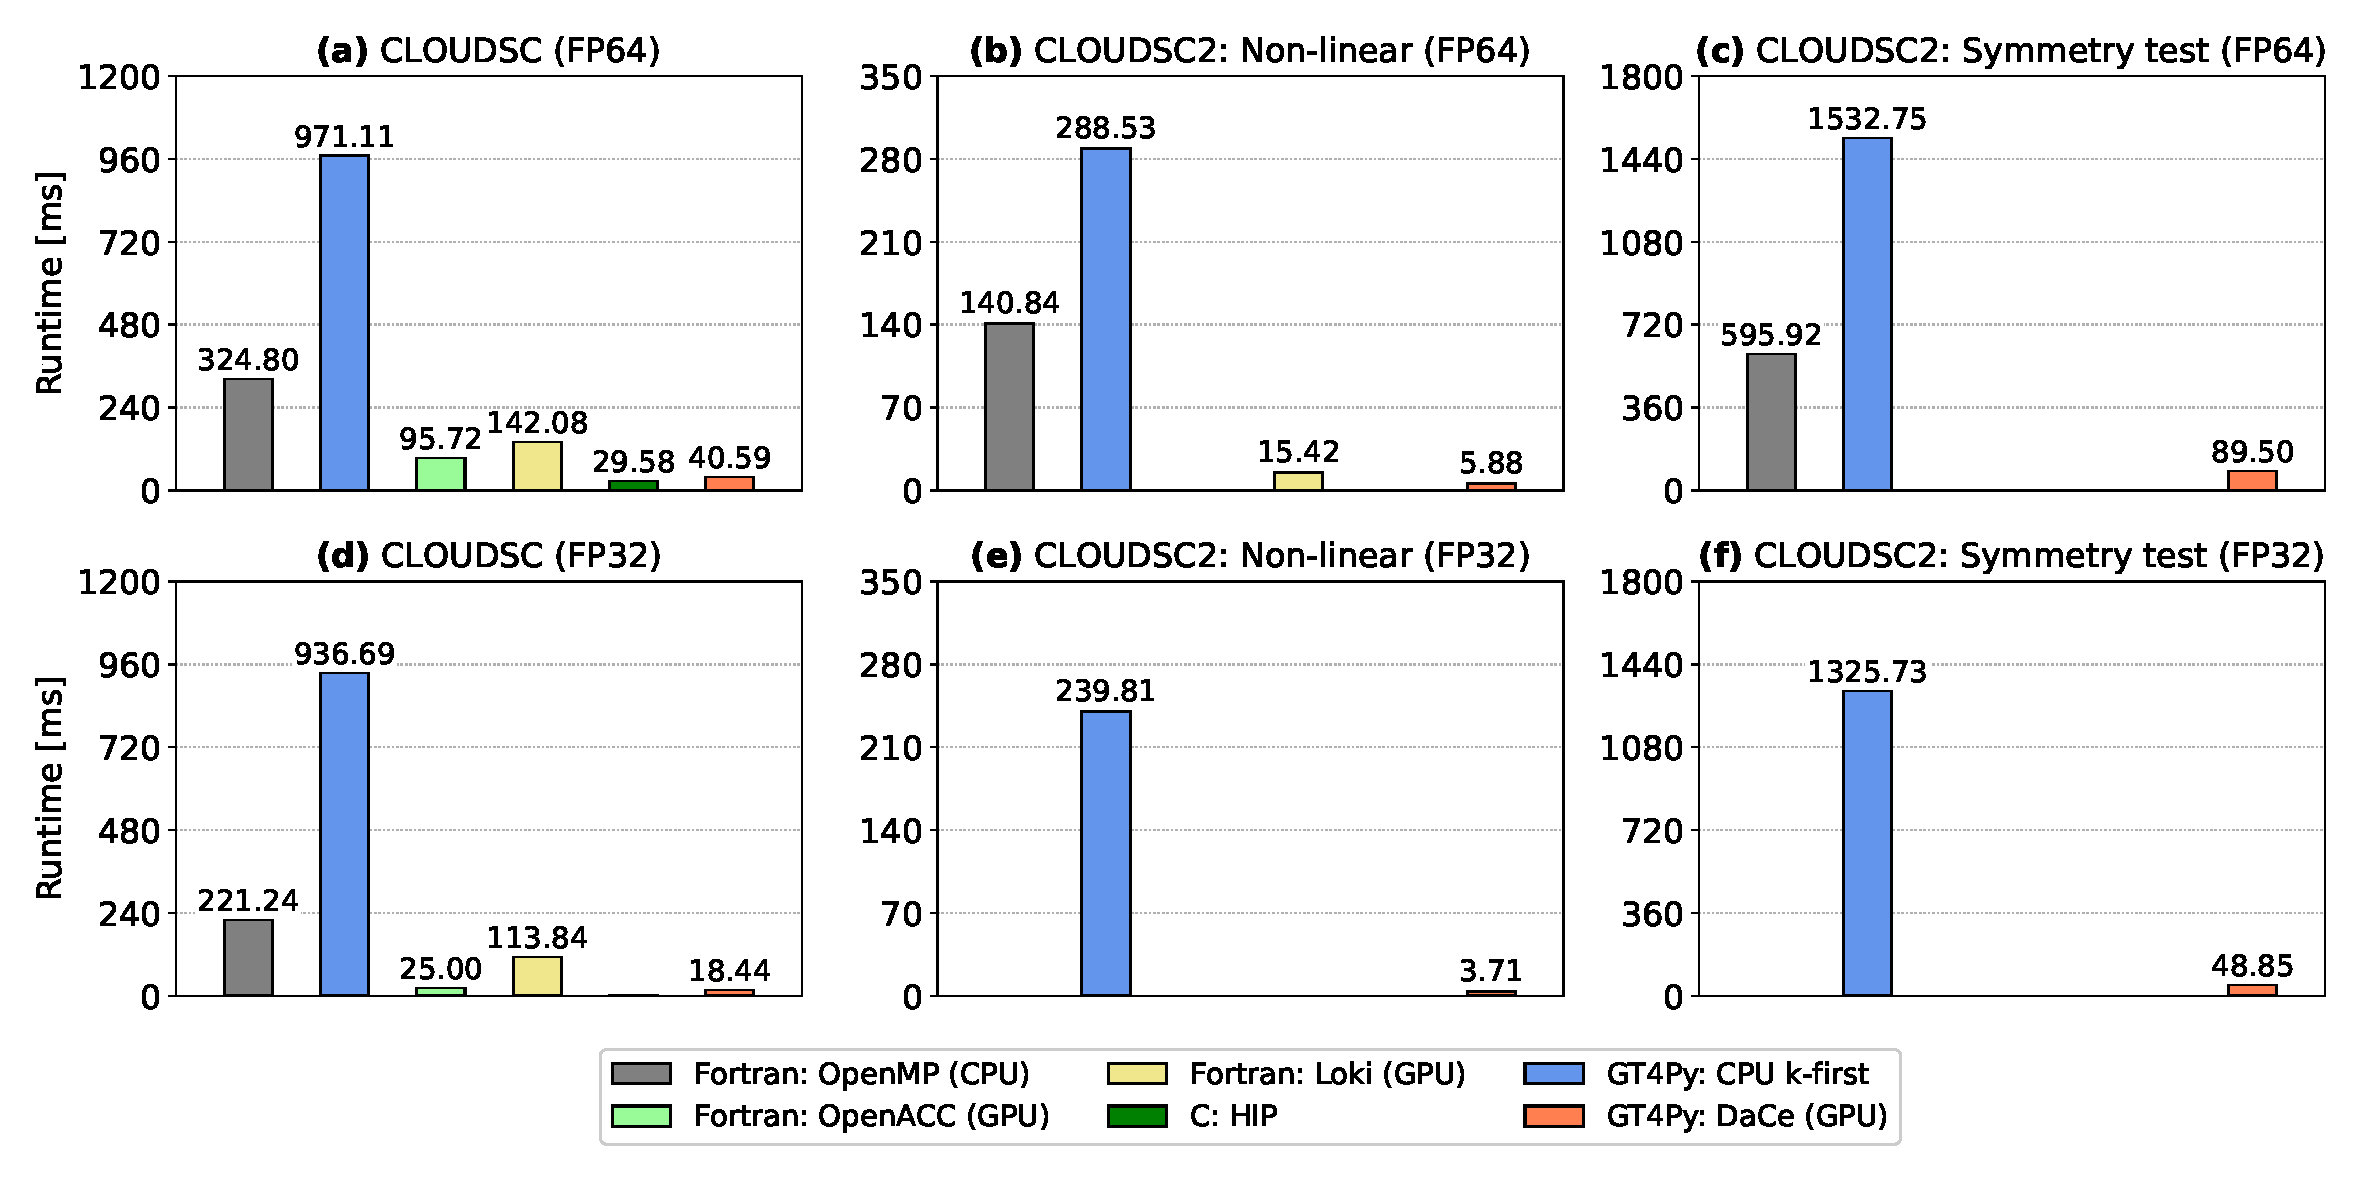
\includegraphics[scale=0.44]{performance_lumi_2.pdf}
            \caption{As Fig.\,\ref{fig:performance-daint} but for the LUMI supercomputer.}
            \label{fig:performance-lumi}
        \end{figure}
        
        The performance of the high-level Python with GT4Py compares well against Fortran with OpenACC. The runtimes for GT4Py with its DaCe backend versus OpenACC are similar on Piz Daint, MeluXina and LUMI. One outlier is the double precision result on LUMI, for which the OpenACC code appears relatively slow. We suppose this behaviour is associated with the insufficient OpenACC support for the HPE Cray compiler. Only the HPE Cray compiler implements GPU offloading capabilities for OpenACC directives on AMD GPUs, meaning that Fortran OpenACC codes require an HPE Cray platform to run on AMD GPUs. In contrast, GT4Py relies on the HIPCC compiler driver developed by AMD to compile device code for AMD accelerators, and this guarantees a proper functioning irrespective of the machine vendor. We further note that the DaCe backend of GT4Py executes roughly two times faster on MeluXina's NVIDIA A100 GPUs than on LUMI's AMD Instinct MI250X GPUs. As mentioned above, from a software perspective, each physical GPU module on LUMI is considered as two virtual GPUs, so that the code is actually executed on half of a physical GPU card. We can therefore speculate that if using both dies of an AMD Instinct MI250X GPU performance would be on par with the NVIDIA A100 GPU.

        Another interesting result is that both CLOUDSC-GT4Py and CLOUDSC2-GT4Py are consistently faster than the implementations generated with Loki. Loki allows to build bespoke transformation recipes to apply changes to programming models and coding styles in an automated fashion. Therefore, GPU-enabled code can be produced starting from the original Fortran by e.g., automatically adding OpenACC directives. However, because not all optimizations are yet encoded in the transformations, the Loki-generated device code cannot achieve optimal performance. Notwithstanding, source-to-source translators such as Loki are of high relevance for enabling GPU execution with large legacy Fortran code bases.

        As used in this paper, GT4Py cannot yet attain the performance achieved by manually optimized native implementations with either Fortran on CPU or CUDA/HIP on GPU. Multi-threaded Fortran can be up to three times faster than the GridTools CPU backend of GT4Py using the k-first (C-like) memory layout, while the DaCe GPU backend of GT4Py can be up to a factor of two slower than CUDA/HIP. On the one hand, so far the development of GT4Py has been focused on GPU execution (see e.g. \cite{dahm23}), because this will be the dominant hardware for time-critical applications in the years to come. On the other hand, we stress that the k-caching CUDA and HIP variants of CLOUDSC were semi-automatically generated by performance engineering experts, starting from an automatic Fortran-to-C transpilation of the SCC variants and manually applying additional optimizations that require knowledge about the specific compute patterns in the application. This process is not scalable to the full weather model and not a sustainable code adaptation method. In contrast, no significant performance engineering (by, e.g., statements fusion and temporaries pruning) has been applied yet with CLOUDSC-GT4Py and CLOUDSC2-GT4Py.

        \begin{figure}[t!]
            \centering
            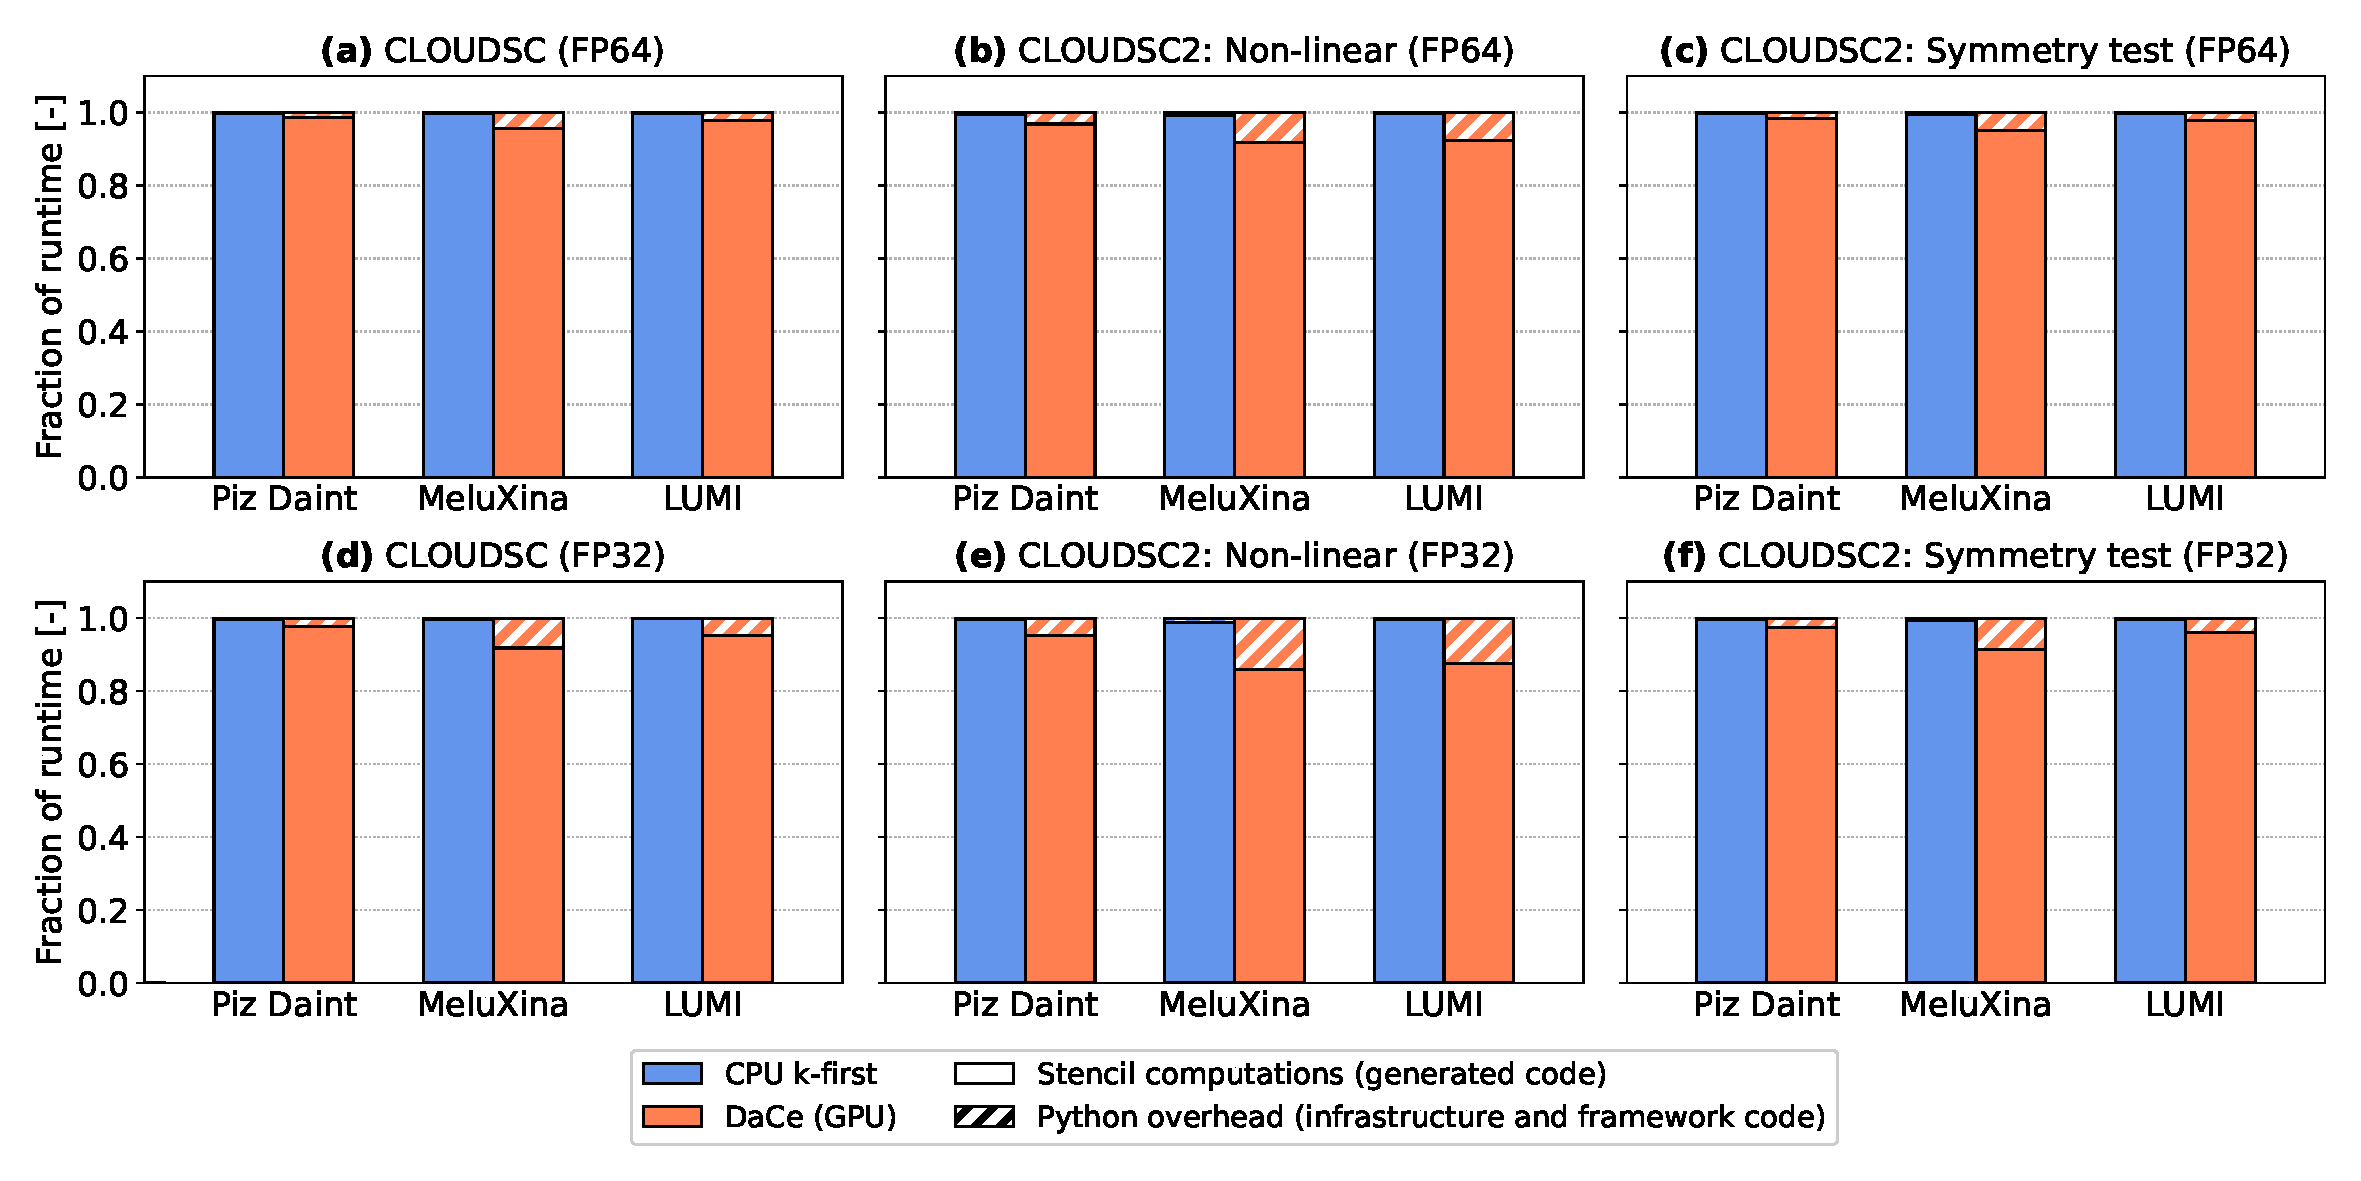
\includegraphics[scale=0.44]{runtime_fraction_1.pdf}
            \caption{For the GT4Py rewrites of CLOUDSC (left column), CLOUDSC2NL (center column) and the symmetry test for CLOUDSC2TL and CLOUDSC2AD (right column), fraction of the total execution time spent within the stencil computations (full bars) and the Python side of the application (hatched bars) on Piz Daint, MeluXina and LUMI. Results are shown for the GridTools C++ CPU backend with k-first data ordering (blue) and the DaCe GPU backend (orange), either using double precision (top row) or single precision (bottom row) floating point arithmetic.}
            \label{fig:runtime-fraction}
        \end{figure}

        To rule out the possibility that the performance gap between the Python DSL and lower-level codes is associated with overhead originating from Python, Fig.\,\ref{fig:runtime-fraction} displays the fraction of runtime spent within the stencil code generated by GT4Py and the high-level Python code of the application (infrastructure and framework code; see Section \ref{section:infrastructure-code}). Across the three supercomputers, the Python overhead decreases as (i) the complexity and length of computations increase, (ii) the peak throughput and bandwidth delivered by the hardware underneath decrease, and (iii) the floating point precision increases. On average, the Python overhead accounts for $5.4\,\%$ of the total runtime on GPU and $0.4\,\%$ on CPU. Interestingly, if one takes into account only the cases for which a working Fortran CPU implementation is available, even if the GT4Py performance was on par with Fortran, the Python overhead would still amount to less than $0.7\,\%$ of the total execution time on average.

        Finally, we observe a significant sensitivity of the GPU performance with respect to the thread block size\footnote{In the Fortran code, the thread block size corresponds to the NPROMA.}: for values smaller than 128, performance is degraded across all implementations, with the gap between CUDA/HIP and GT4Py+DaCe being smaller. This shows that some tuning and toolchain optimizations can be performed to improve performance with the DSL approach.

    %\biblio
\end{document}